\documentclass[8pt]{beamer}

\usetheme{metropolis}
\metroset{sectionpage=none}
\setbeamertemplate{headline}{
  \begin{beamercolorbox}[wd=\paperwidth,ht=2.25ex,dp=1ex]{palette primary}
    \hfill\insertsection\hspace*{2em}
  \end{beamercolorbox}
}
\usepackage{graphicx} % Per includere immagini
\usepackage{listings} % Per il codice sorgente
\usepackage{textcomp} % Per simboli come il carattere di virgoletta singola diritta

% --- Informazioni Tesi ---
\title{Sviluppo di un pannello Web a supporto di un filtro DNS per malware e contenuti}
\subtitle{Un'architettura a servizi che si inserisce nel contesto aziendale esistente}
\date{II Sessione di Laurea, A.A. 2024-2025}
\author{Alessandro Valmori}
\institute{Università di Bologna \and Relatore: Prof. Mirko Viroli \and Correlatore: Dott. Nicolas Farabegoli}


% --- Stile per il codice ---
\definecolor{codegreen}{rgb}{0,0.6,0}
\definecolor{codegray}{rgb}{0.5,0.5,0.5}
\definecolor{codepurple}{rgb}{0.58,0,0.82}
\definecolor{backcolour}{rgb}{0.95,0.95,0.92}

\lstdefinestyle{mystyle}{
    backgroundcolor=\color{backcolour},   
    commentstyle=\color{codegreen},
    keywordstyle=\color{magenta},
    numberstyle=\tiny\color{codegray},
    stringstyle=\color{codepurple},
    basicstyle=\ttfamily\footnotesize,
    breakatwhitespace=false,         
    breaklines=true,                 
    captionpos=b,                    
    keepspaces=true,                 
    numbers=left,                    
    numbersep=5pt,                  
    showspaces=false,                
    showstringspaces=false,
    showtabs=false,                  
    tabsize=2,
    literate=
      {'’'}{{\textquotesingle}}1
      {'`'}{{\textquotesingle}}1
}
\lstset{style=mystyle}

\begin{document}

% --- SLIDE 1: TITOLO ---
\maketitle


% --- INIZIO SEZIONI ---

\section{Contesto e Obiettivi}

\begin{frame}{Contesto e Motivazione}
  \begin{block}{Problema Aziendale }
    FlasStart Group S.r.l., durante un re-engineering della piattaforma, necessitava di una soluzione "ponte" per fornire ai clienti una dashboard di analisi dati in modalità \textbf{readonly}.
  \end{block}
  \begin{block}{Obiettivo del Progetto }
    Sviluppare uno \textit{spike tecnologico} per colmare questa lacuna funzionale immediata, in attesa del rilascio della nuova infrastruttura a Novembre 2025.
  \end{block}
  \begin{alertblock}{Obiettivo della Tesi }
    Analizzare come i principi della programmazione a oggetti guidino le scelte architetturali in un progetto industriale con vincoli reali.
  \end{alertblock}
\end{frame}

\section{Architettura e Design}

\begin{frame}{Architettura di Alto Livello}
  \begin{figure}
    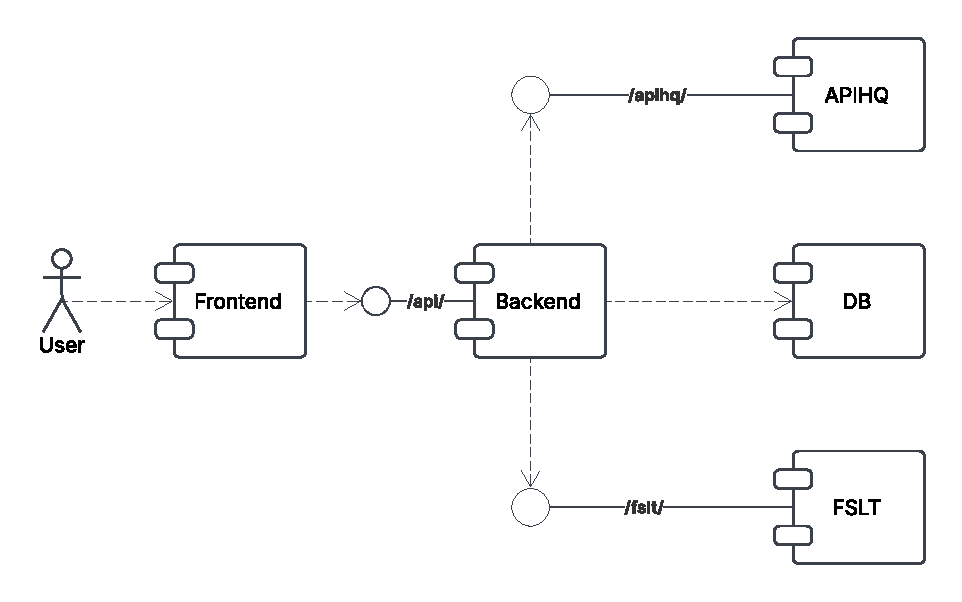
\includegraphics[width=0.5\textwidth]{figures/components.pdf}
  \end{figure}
  \begin{itemize}
    \item \textbf{Frontend (React)}: Unico punto di contatto per l'utente.
    \item \textbf{Backend (Java + Spring WebFlux)}: Nucleo logico, API Gateway e gestore dell'autenticazione.
    \item \textbf{Database (PostgreSQL)}: Persistenza dei soli dati applicativi (utenti, sessioni).
    \item \textbf{API Esterne}: Integrazione con due servizi legacy di FlashStart.
  \end{itemize}
\end{frame}

\begin{frame}{Design del Backend: Struttura e Reattività}
  \frametitle{Design del Backend: Struttura e Reattività}
  \begin{columns}[T]
    \column{0.5\textwidth}
    \begin{block}{Architettura a Strati}
      Adottata un'architettura a 3 strati per una netta \textbf{separazione delle responsabilità}:

    \end{block}
    \begin{figure}
      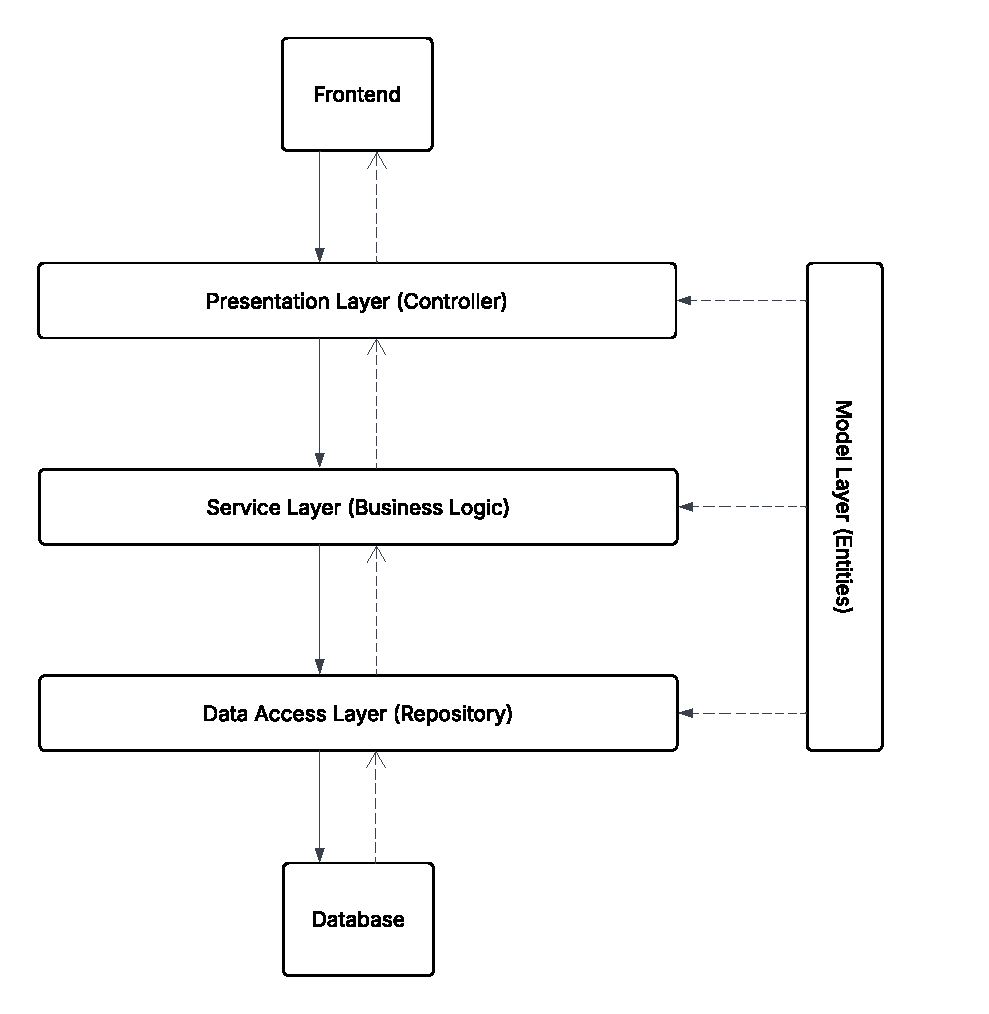
\includegraphics[width=\textwidth]{figures/layer_design.pdf}
    \end{figure}

    \column{0.5\textwidth}
    \begin{alertblock}{Programmazione Reattiva}
      \textbf{Problema}: Il backend funge da gateway e deve gestire numerose chiamate di I/O (API esterne, DB) senza bloccarsi.
      \vspace{0.5cm}

      \textbf{Soluzione}: L'uso di \textbf{Spring WebFlux} con un event loop non bloccante.
      \begin{itemize}
        \item Permette di gestire un alto numero di connessioni concorrenti con poche risorse.
        \item Ideale per carichi di lavoro I/O-bound, garantendo scalabilità e resilienza.
      \end{itemize}
    \end{alertblock}
  \end{columns}
\end{frame}

\begin{frame}[fragile]{Comunicazione Robusta: Decorator con Intercettori}
  \frametitle{Comunicazione Robusta: Decorator con Intercettori Axios}
  \begin{columns}[T]
    \column{0.5\textwidth}
    \begin{alertblock}{Problema}
      Come centralizzare la logica trasversale delle chiamate API (aggiungere token, gestire errori) senza duplicare codice nel frontend?
    \end{alertblock}

    \begin{block}{Soluzione: Pattern Decorator}
      Sfruttando gli \textbf{intercettori} di Axios, ogni chiamata API viene "decorata" dinamicamente con funzionalità aggiuntive:
      \begin{itemize}
        \item \textbf{Intercettore di Richiesta}: Aggiunge l'header \texttt{Authorization} a ogni chiamata in uscita.
        \item \textbf{Intercettore di Risposta}: Cattura gli errori \texttt{401 Unauthorized} e gestisce in modo trasparente il flusso di rinnovo del token.
      \end{itemize}
    \end{block}

    \column{0.5\textwidth}
    \begin{figure}
      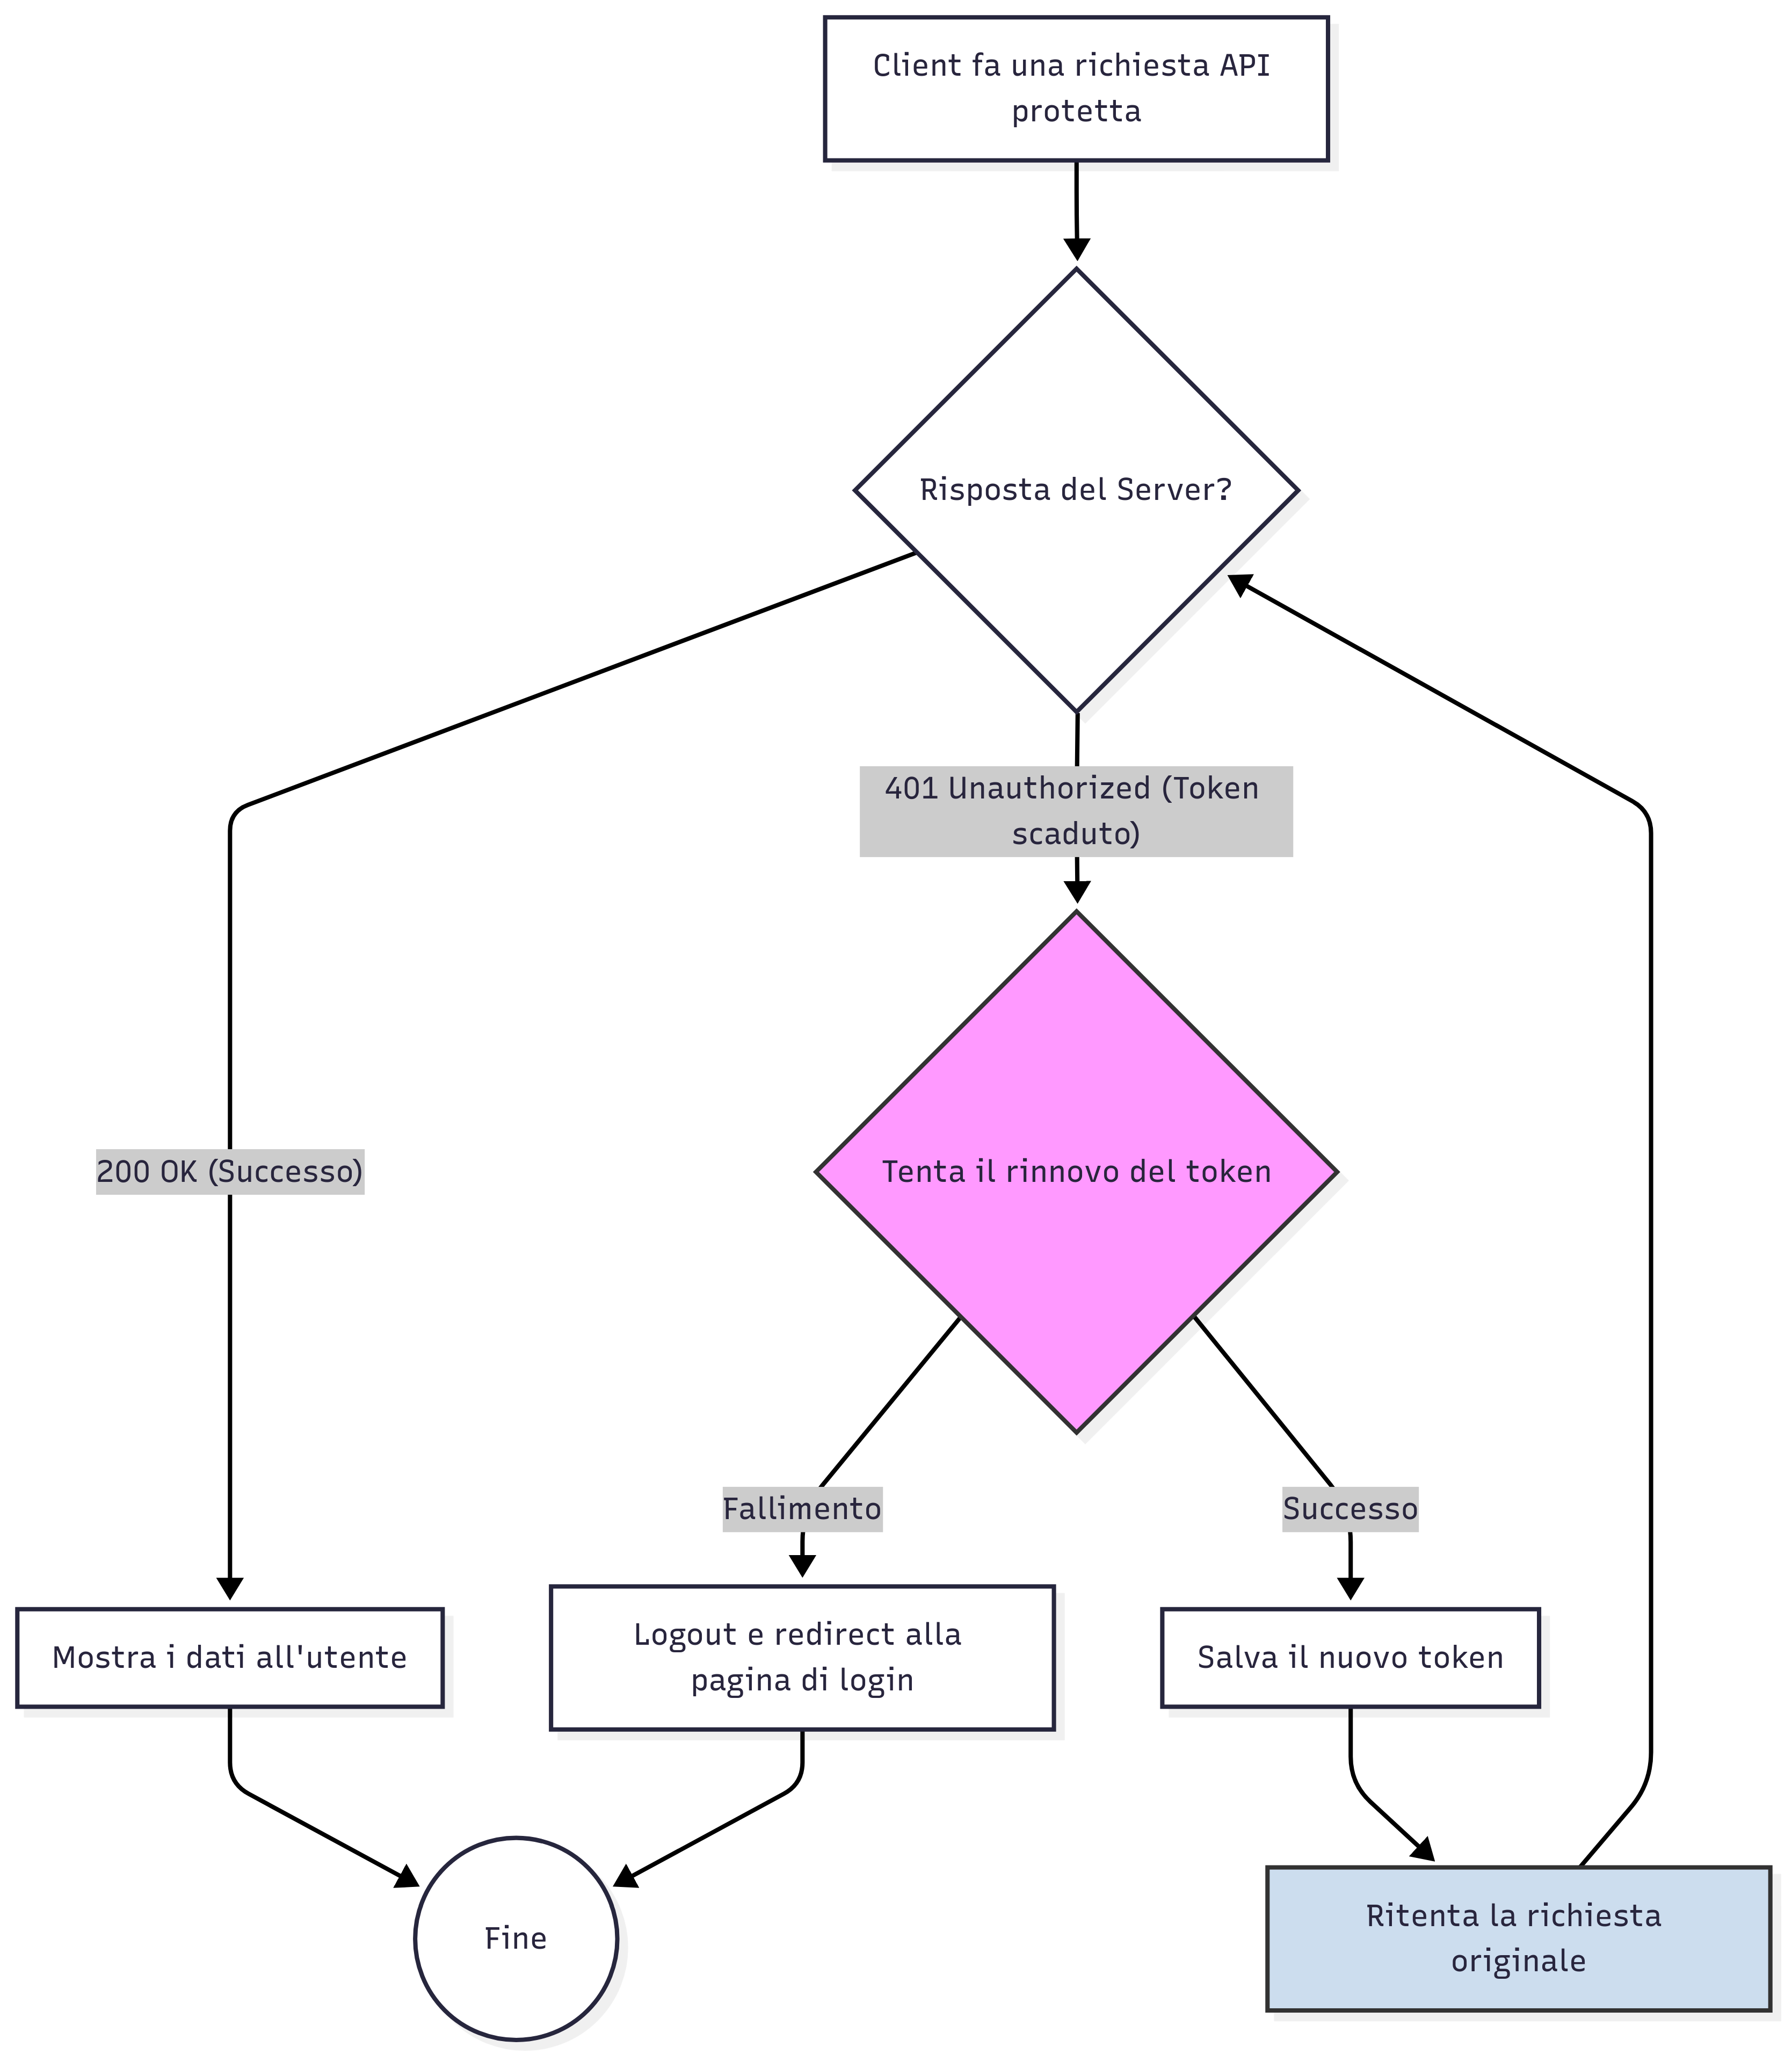
\includegraphics[width=\textwidth]{figures/axios_flow.png}
    \end{figure}
  \end{columns}
\end{frame}

\section{Implementazione e Risultati}

\begin{frame}{Flusso di Sicurezza: Autenticazione Stateless Robusta}
  \frametitle{Flusso di Sicurezza: Autenticazione Stateless Robusta}

  \begin{block}{Principio Guida}
    L'architettura di autenticazione è \textbf{stateless} e basata su JSON Web Tokens (JWT), con un design mirato a mitigare i rischi legati al furto di credenziali.
  \end{block}

  \begin{columns}[T]
    \column{0.5\textwidth}
    \begin{exampleblock}{I Token e i Loro Ruoli}
      \begin{itemize}
        \item \textbf{Access Token}:\\Ha una vita breve (15 min) per minimizzare l'esposizione. Viene trasmesso nel corpo della risposta e gestito in memoria dal client.

        \item \textbf{Refresh Token}:\\Ha una vita lunga (7 giorni) per la persistenza della sessione. È archiviato in un cookie sicuro \texttt{HttpOnly}.
      \end{itemize}
    \end{exampleblock}

    \column{0.5\textwidth}
    \begin{alertblock}{Misure di Sicurezza Chiave}
      \begin{itemize}
        \item \textbf{Cookie HttpOnly}:\\Il Refresh Token non è accessibile via JavaScript, proteggendolo da attacchi XSS.

        \item \textbf{Token Rotation}:\\Il Refresh Token è \alert{monouso}. Ad ogni utilizzo, viene invalidato e sostituito, una misura fondamentale contro gli attacchi di tipo *replay*.

        \item \textbf{Rinnovo Trasparente}:\\Un intercettore (pattern \textit{Decorator}) gestisce il rinnovo dei token in modo automatico e invisibile all'utente.
      \end{itemize}
    \end{alertblock}
  \end{columns}
\end{frame}

\begin{frame}{Infrastruttura e Automazione (CI/CD)}
  \frametitle{Infrastruttura e Automazione (CI/CD)}

  % --- PARTE SUPERIORE: DUE COLONNE ---
  \begin{columns}[T]
    % --- Colonna Sinistra: Testo ---
    \column{0.4\textwidth}
    \begin{block}{Automazione del Rilascio}
      Implementata una pipeline di CI/CD ibrida per automatizzare l'intero ciclo di vita del software.
    \end{block}

    \textbf{Stack Tecnologico:}
    \begin{itemize}
      \item \textbf{Orchestrazione}: GitHub Actions.
      \item \textbf{Esecuzione}: Self-Hosted Runner.
      \item \textbf{Artefatti}: Immagini Docker.
    \end{itemize}

    % --- Colonna Destra: Figura ---
    \column{0.6\textwidth}
    \begin{figure}
      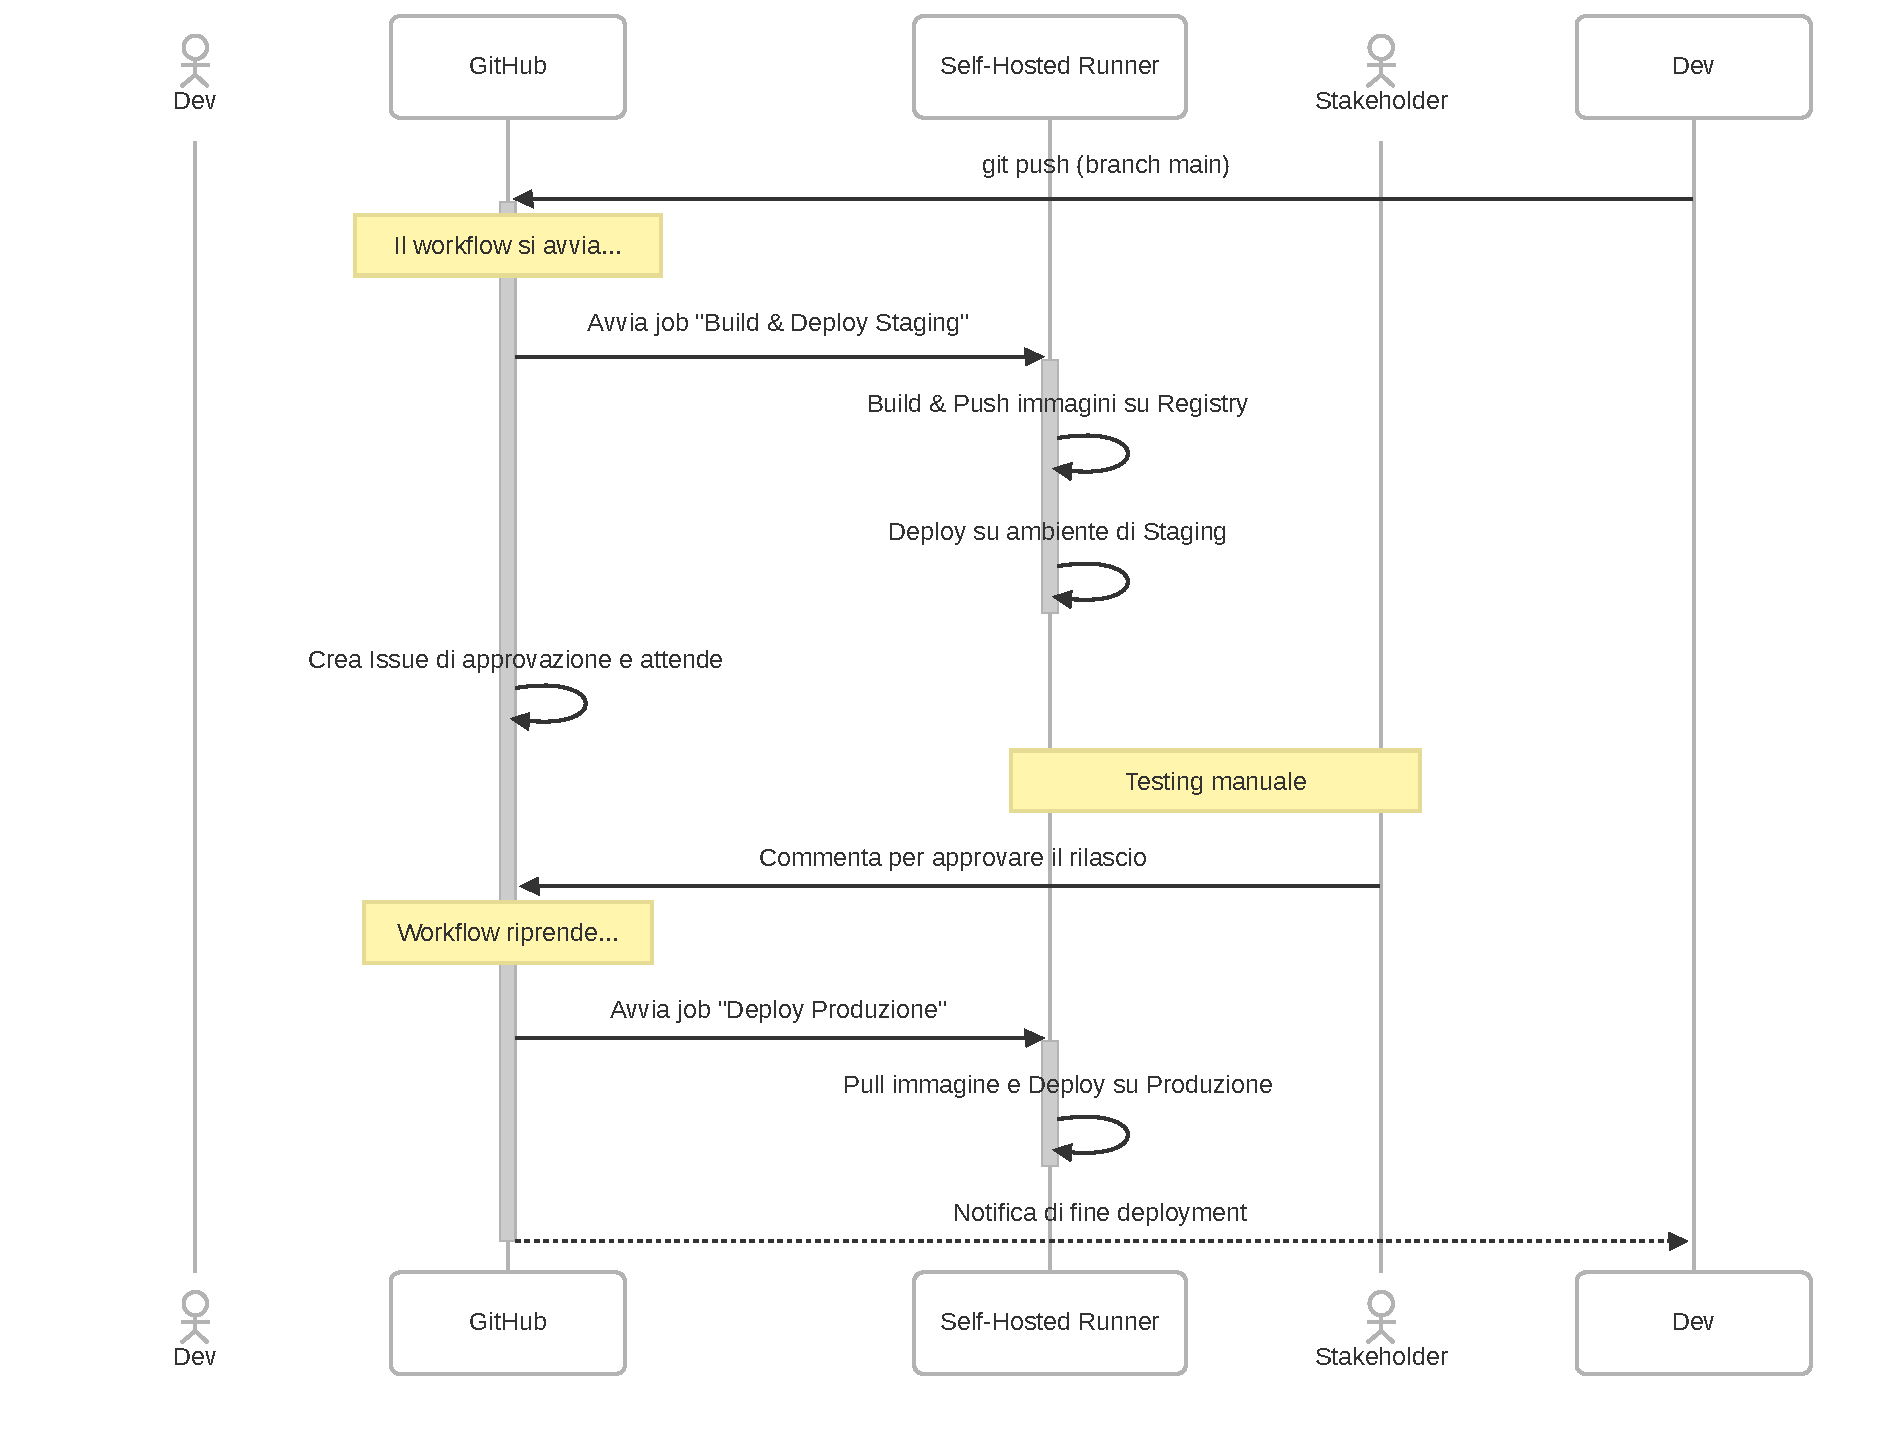
\includegraphics[width=\textwidth]{figures/pipeline_sequence.pdf}
    \end{figure}
  \end{columns}

  \vfill % Aggiunge spazio verticale flessibile

  % --- PARTE INFERIORE: FLUSSO ORIZZONTALE ---
  \begin{center}
    \begin{figure}
      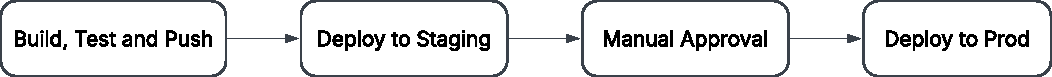
\includegraphics[width=\textwidth]{figures/workflow.pdf}
    \end{figure}
  \end{center}

\end{frame}

\section{Conclusioni}

\begin{frame}{Conclusioni e Risultati}
  \begin{block}{Risultati del Progetto}
    L'obiettivo è stato pienamente raggiunto: è stata sviluppata un'applicazione web full-stack che ha soddisfatto un'esigenza di business critica e immediata.
  \end{block}

  \begin{exampleblock}{Impatto e Adozione}
    La stabilità e l'efficacia della soluzione sono testimoniate dalla sua adozione in produzione da parte di clienti internazionali come \textbf{Telefónica} e un importante \textbf{Carrier Tier-1} statunitense.
  \end{exampleblock}

  \begin{alertblock}{Apprendimento Chiave}
    Il progetto ha dimostrato come l'applicazione rigorosa dei principi e dei design pattern della programmazione a oggetti sia cruciale per creare software robusto e manutenibile, anche in un contesto industriale agile e con vincoli di tempo stringenti.
  \end{alertblock}
\end{frame}


\end{document}